\documentclass{article}
\usepackage[utf8]{inputenc}
\usepackage[a4paper, left=1.1in,right=1.1in,top=1.1in,bottom=0.9in ]{geometry}
\usepackage{bera}
\usepackage{wrapfig}
\usepackage{hyperref}
\usepackage{amsfonts, amsmath, amssymb}
\usepackage{fancyhdr}
\usepackage{multicol}
\usepackage{luacode}
\usepackage[dvipsnames]{xcolor} 
\usepackage[document]{ragged2e}
\justifying
\usepackage[dvipsnames]{xcolor}
\usepackage[none]{hyphenat}
\usepackage[utf8]{inputenc}
\makeatletter
\setlength{\@fptop}{0pt}
\makeatother
\usepackage{float}
\usepackage[T1]{fontenc}
\usepackage{graphicx}
\usepackage{listings}
\pagestyle{fancy}
\fancyhead[L]{\slshape \MakeUppecase INFO}
\fancyhead[R]{\MakeUppecase Alberto Mondino}







\title{JSON}\fancyfoot[]{}
\author{Alberto Mondino}
\fancyfoot[C]{\thepage}
\renewcommand{\footrulewidth}{0.9pt}

\begin{document}
\begin{titlepage}
\begin{center}
\vspace*{1cm}

\vfill
\line(1,0){400}


\Huge\textbf{INFO}

\normalsize\textbf{\textit{-anche se fatto male-}}

\line(1,0){400}
\vfill
\textbf{Alberto Mondino}


\end{center}
\end{titlepage}

\tableofcontents

\newpage
\section{\underline{Basi di dati}}

\textbf{\underline{DATO}}:I dati sono rappresentazioni originarie, non
interpretate, di un valore.
\\ \textbf{\underline{INFORMAZIONE}}:
L’informazione deriva da un dato, o da un insieme di dati, che sono
stati contestualizzati, interpretati in modo da essere significativi.
\subsection{I dati in azienda}
\subsubsection{L'azienda}
In economia il \textit{\textbf{Know-How}} è un fattore chiave. per il successo di un'azienda \\ Il \textit{Know-How} non sono altro che le conoscenze aziendali e la loro gestione.
\subsubsection{Le decisioni}
In azienda esistono tre decisioni:
\begin{enumerate}
    \item \textbf{\underline{Strategiche}}: definiscono le linee globali dell'azienda, sono prese a livello \textit{dirigenziale}
    
    \item \textbf{\underline{Tattiche}}: riguardano l'attuazione delle decisioni strategiche, prese dai quadri \textit{intermedi }
    \item\textbf{\underline{Operative}}:riguardano la gestione delle risorse, prese dal personale \textit{esecutivo}
\end{enumerate}


\begin{center}
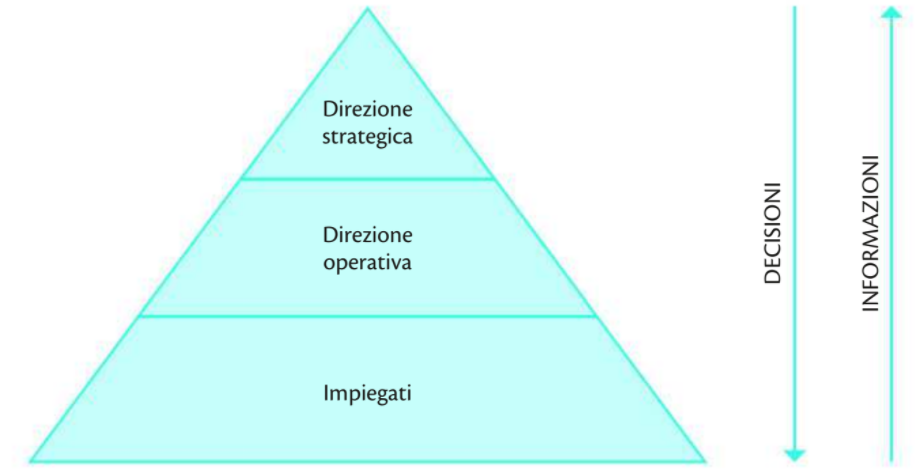
\includegraphics[h, scale=0.7]{pir.PNG}
\end{center}
\subsubsection{Il flusso informativo}
Il flusso informativo riguarda tutti i dati e informazioni necessari all'azienda, dati che devono arrivare dove necessario affidabilmente.


In azienda il flusso delle informazioni prevede due casi
\begin{itemize}
    \item \textbf{Push}:l'informazione viene inviata a tutti, anche a chi non ne ha bisogno
    \item \textbf{Pull}: l'informazione è messa a disposizione in database accesso agli utenti
\end{itemize}
\begin{figure}[h!]
    \centering
    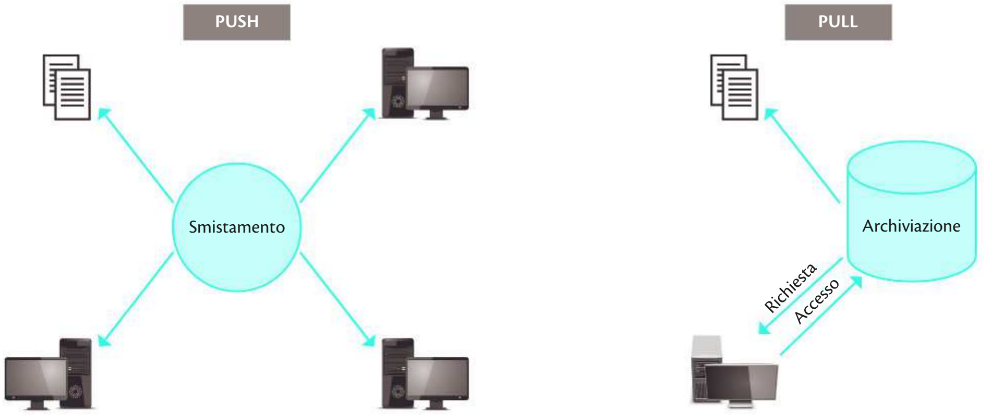
\includegraphics[width=10cm]{Untitled picture.png}
\end{figure}
\subsection{Il sistema informativo aziendale}
\subsubsection{Il sistema informativo}
\underline{\textbf{Sistema Informativo}}: organizza e gestisce le informazioni aziendali, si occupa delle comunicazioni dell'azienda. Il sistema informativo è formato da tutte le persone che lavorano nell'azienda e tutte le procedure necessarie per l'elaborazione dei dati.
\subsubsection{Sistema informatico}
\begin{figure}[h!]
    \centering
    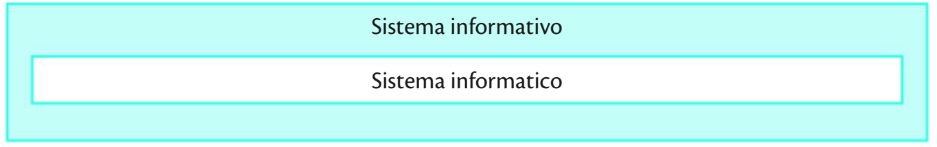
\includegraphics[width=10cm]{Untitled picture1.png}
\end{figure}

\underline{\textbf{Il sistema informativo}} automatizzato è l'insieme di tecnologie hardware e software che permettono l'automatizzazione delle funzioni informative aziendali, riducendo gli errori umani, elaborando e smistando le informazioni.

\subsection{Memorizzare dati}
\subsubsection{I File}
I file consentono la conservazione dei dati, ne esistono diverse tipologie:
\begin{itemize}
    \item \textbf{\underline{file di testo}}: sequenze di caratteri ASCII, organizzate per righe 
    \item \textbf{\underline{file binari}}
    \item \textbf{\underline{file strutturati}}: insieme di record memorizzati in codifica binaria. 
\end{itemize}
\subsubsection{File strutturati}
Un archivio o file è un insieme di record memorizzati su un supporto di memoria permanente.

\begin{center}
    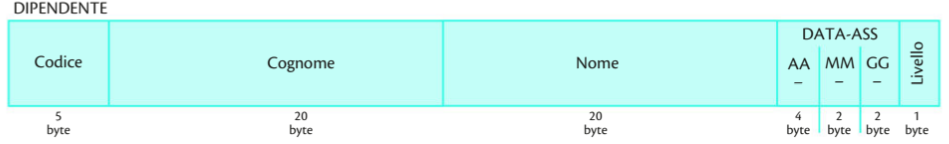
\includegraphics[h, scale=0.9]{rec.PNG}
\end{center}

Per ottimizzare la ricerca tra i record si utilizza una \textbf{chiave primaria}, scelta tra le chiavi candidate, che identifica univocamente ciascun record. I valori assunti dalla chiave primaria devono essere tutti diversi.
\\
Tipi di chiavi primarie:
\begin{itemize}
    \item \textbf{chiave naturale}: chiavi che hanno un collegamento logico con il mondo (CF)
    \item \textbf{chiave surrogata}: chiave che non ha nessun collegae+mento logico con il mondo, ma che viene calcolata dal DBMS esclusivamente per identificare univocamente i record.
\end{itemize}

\subsection{Dal file system alle basi di dati}
\subsubsection{Il sistema EDP}
Il sistema \textbf{EDP}(\textbf{E}lectronic \textbf{D}ata \textbf{P}rocessing) è un insieme di dati memorizzati su supporti elettronici e di applicazioni informatiche.
La gestione dei dati è affidata al file system.

All'interno del sistema EDP è presente un analista che ha il compito di rendere l'applicazione il più effice possibile. Nel sistema EDP ogni applicazione opera in modo indipendente dalle altre applicazioni, facendo uso dei propri dati e dei propri programmi.

\begin{center}
    
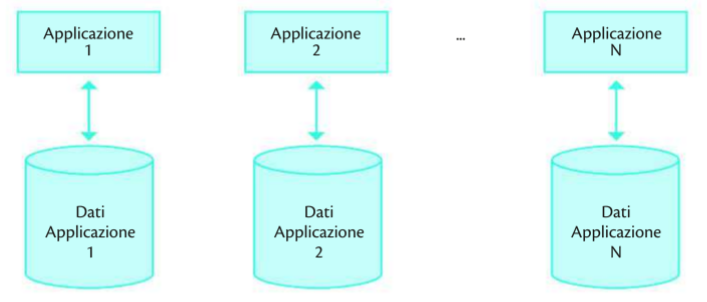
\includegraphics[h, scale=1]{edp.PNG}

\end{center}%%%%%%


\subsubsection{Basi di dati e DBMS}
Una base di dati è una collezione di dati strutturati, progettati per essere usati in applicazioni differenti e da utenti differenti. È un insieme di dati memorizzati senza senza duplicazioni inutili per servire più applicazioni in contemporanea, organizzati in modo da essere indipendenti dai programmi che li usano.

\subsubsection{Vantaggi nell'uso dei DB}
Vantaggi nell'uso dei DB rispetto ai file e rispetto a EDP:
\begin{itemize}
    \item \textbf{Eliminazione} delle \textbf{ridondanze}, evitare duplicazioni delle informazioni
    \item \textbf{Eliminazione} delle \textbf{inconsistenze}, quando due dati che rappresentano la stessa informazione hanno due valori diversi
    \item Integrità dei dati, i dati infatti vengono protetti da cambiamenti non autorizzati o non corretti
\end{itemize}

\subsection{Architettura}
\subsubsection{Il modello ANSI/SPARC}
\textbf{ANSI/SPARC} è dodato di tre livelli: esterno, logico e interno, che permettono ai DBMS di nasconedere l'organizzazione dei dati.

\begin{center}
    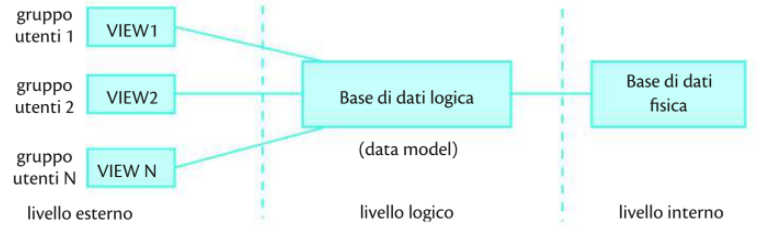
\includegraphics[h]{ansi.PNG}
\end{center}


\begin{itemize}
    \item \textbf{Livello esterno}: detto anche livello applicativo, descrive i dati come sono visti da una o più applicazioni. Possono esistere più schemi esterni (o sottoschemi) che riguardano la "Vista" di interesse per ogni singola applicazione. Semplifica il lavoro agli utenti, mostrando loro solamente la parte che gli interessa con una rappresentazione più familiare e semplice dei dati.
    \item \textbf{Livello logico}: Descrive formalmente tutti gli oggetti di interesse per le applicazioni, offrendo una rappresentazione precisa e dettagliata delle strutture dati(record, campi, chiavi) necessarie per memorizzare informazioni. Permette sia l'aggiunta che la modifica di sottoschemi senza impatto sullo schema concettuale e offre uno strumento di controllo sul contenuto e sull'utilizzo del DB.
    \item \textbf{Livello interno}: Rappresenta la descrizione formale delle strutture fisiche degli archivi che costituiscono il DB.
\end{itemize}

\subsubsection{Indipendenza logica e fisica}
Per \underline{\textbf{indipendenza logica}} si intende la possibilità di modificare lo schema logico senza che vada ad  influenzare i programmi che si interfacciano con quella base di dati.
%

Per \underline{\textbf{indipendenza fisica}} si intende la possibilità di modificare l'organzzazione fisica dei dati, senza dover modificare l'organizzazione logica.

\subsection{Linguaggi e utenti}
\subsubsection{Linguaggi per i database}
Per poter gestire le basi di dati tramite il DBMS si fa uso di due tipologie di linguaggi:DDL e DML.
\subsubsection{DDL}
\textbf{DDL} (\textbf{D}ata \textbf{D}efinition \textbf{L}anguage), serve per la definizione dello schema logico. Consente di definire i tipi di entità presenti nello schema concettuale e le loro relazioni. Serve anche per definire eventuali viste (sottoschemi), che consentono di selezionare solo la parte dello schema che interessa. Utilizzato principalmente dai DBA.

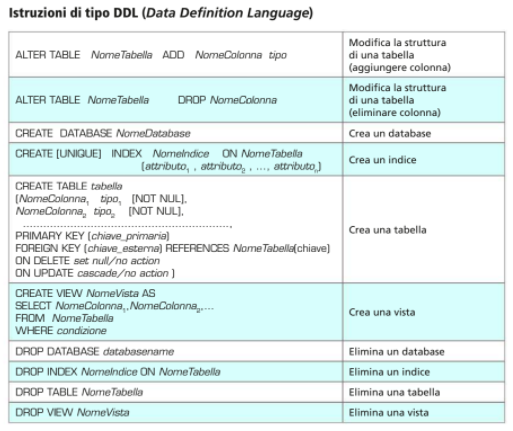
\includegraphics[scale=1.5]{ddl1.PNG}



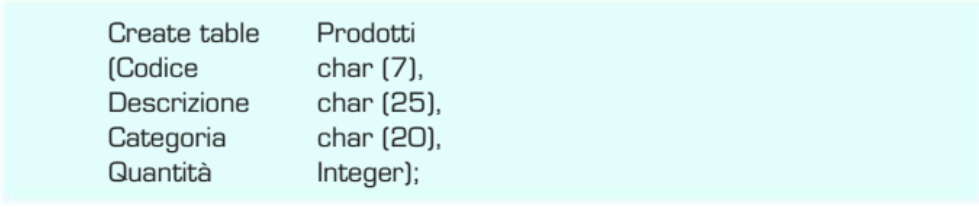
\includegraphics[h, scale=0.8]{ddl.PNG}    



\subsubsection{DML}
 \textbf{DML} (\textbf{D}ata \textbf{M}anipulation \textbf{L}anguage), utilizzato per inserire, modificare e cancellare le informazioni contenute all'interno del DB. I DML forniscono all'utente uno strument per interrogare e modificare le informazioni contenute nel DB.
 \begin{itemize}
     \item procedurali: quando hanno gli operatori per trattare i singoli record
     \itemnon procedurali: quando gli operatori non hanno il cocetto di posizione
 \end{itemize}
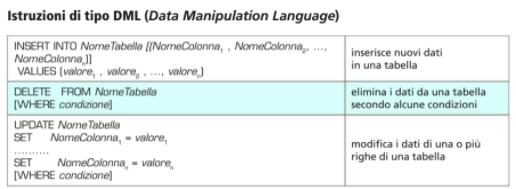
\includegraphics[scale=1.6]{dml.PNG}
\\
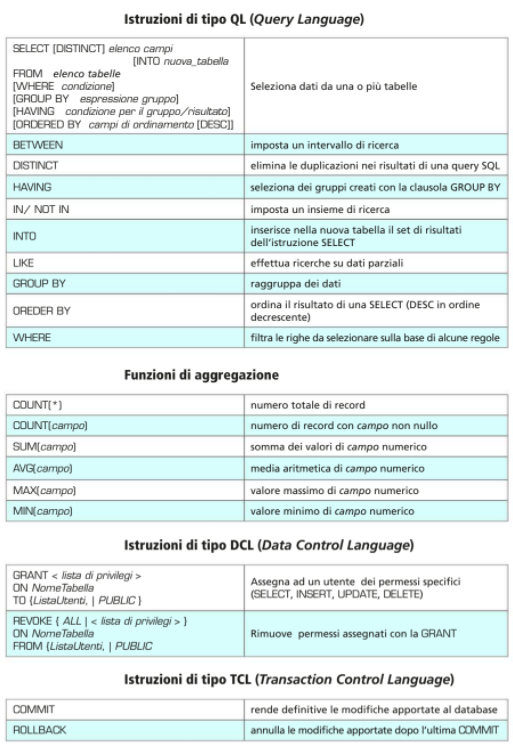
\includegraphics[scale=1.6]{comandi.PNG}

\subsubsection{Gli utenti}
\begin{itemize}
    \item \textbf{\underline{DBA}}\begin{itemize}
        \item creare e mantenere lo schema logico
        \item definire e mantenere lo schema interno
        \item definire e se necessario aggiornare i diritti di accesso (gran e revoke)
        \item ripristinare la base di dati in caso di malfunzionamento
    \end{itemize}
    \item \textbf{\underline{programmatori}}: realizzano applicazioni utilizzando un DML.
    \item \textbf{\underline{utenti finali}}: interagiscono col DB tramite delle maschere con interfaccia grafica
\end{itemize}
\subsection{Sicurezza nelle basi di dati}
\subsubsection{Problematiche di sicurezza}
Le problematiche legate alla sicurezza sono di fondamentale importanza, un DBMS è sviluppato per tenere sotto controllo l'aspetto della privatezza, integrità e consistenza dei dati.
\subsubsection{Privatezza}
La privatezza riguarda la gestione dei permessi di accesso in un DB, è necessario garantire la possibilità a chi è autorizzato, e contemporaeamente negare l'accesso a chi non ne ha diritto.

\begin{enumerate}
    \item Il DBA stabilisce le autorizzazioni (solo lettura, solo scrittura, ecc.) tramite il DDL. (grant e revoke)(esempio della banca)
    \item Questo controllo deve essere constantemente effettuato, ad ogni richiesta il DBMS deve controllare che il richiedete abbia effettivamente i permessi per accedere ad una risorsa.
\begin{center}
    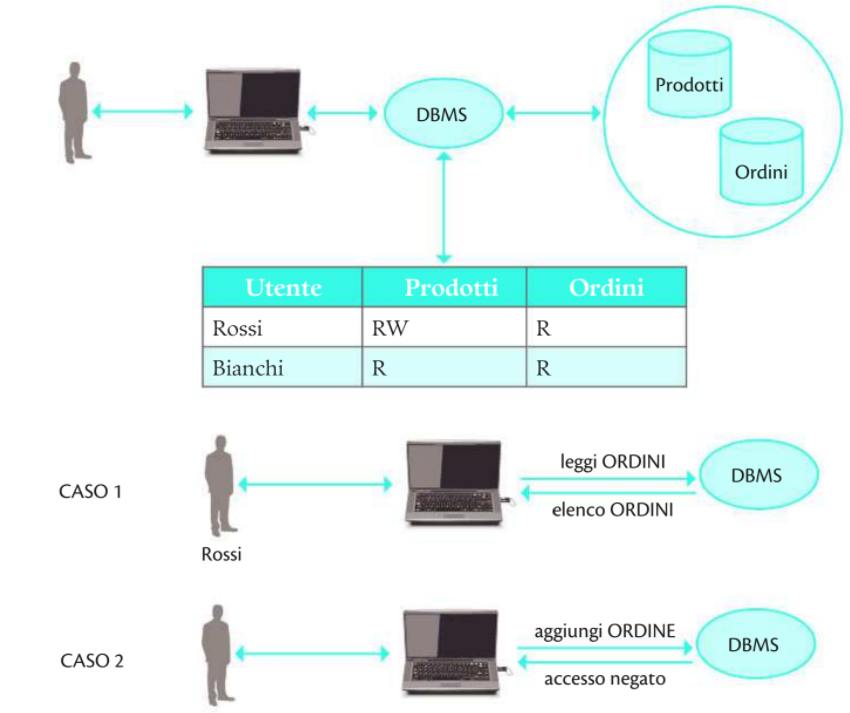
\includegraphics[h, scale=0.8]{privatezza.PNG}
\end{center}

\end{enumerate}

\subsubsection{Vincoli di integrità}
Il vincolo di integrità riguarda le relazioni esistenti tra i dati. La gestione delle informazioni deve essere sicura e corretta, ed un aspetto da controllare è la protezione contro l'aggiornamento errato del database. Per evitare questa complicazione vengono definiti dei \textbf{vincoli intra-relazionali}, che possono riguardare solo un entità (vincoli di unicità, vincoli di dominio), oppure possono definire più entità contemporaneamente.

I vincoli di integrità vengono definiti dal DBA.

\subsubsection{Vincolo di integrità referenziale}
Riguarda il controllo di entità che risultano correlate, anche se memorizzate su archivi diversi.
Il libro fa l'esempio di un operazione su conto corrente: dobbiamo evitare che eventuali prelievi e versamenti vengano effettuati su conti correnti inesistenti. 


\subsubsection{Vincoli di dominio}
I vincoli di dominio definiscono il campo di esistenza di un attributo. Definiscono delle regole da rispettare relative ad attributi. Ad esempio il libro fa l'esempio dell'età, infatti se stiamo definendo l'età di una persona, il vincolo sarà quello di non permettere età minori di 0.
\\
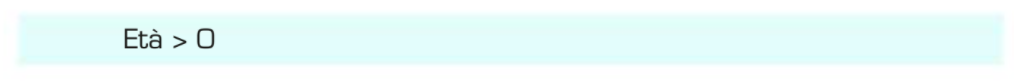
\includegraphics[h]{eta.PNG}
\\ oppure 
\\
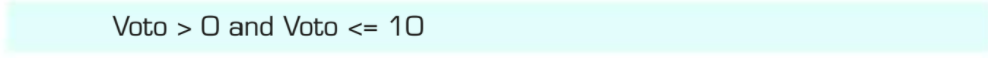
\includegraphics[h]{voto.PNG}
\\

\subsubsection{Vincoli di relazione}
Esprimono condizioni sui valori assunti tra i campi con delle relazioni. 

\begin{footnotesize}

esempi:\\
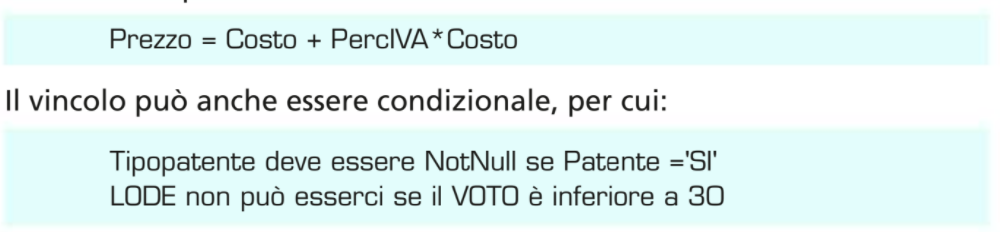
\includegraphics[h, scale=0.8]{vincolo.PNG}
\end{footnotesize}

\subsubsection{Consistenza della base di dati}
La coerenza dei dati è legata al controllo di validità che a sua volta si lega alla modifica contemporanea di dati collegati.

Una \textbf{transazione} è un insieme di istruzioni che formano un'unità di lavoro indivisibile. La transazione deve iniziare e terminare con il DB in uno stato consistente.
\\
Una base di dati si dice \textit{consistente} quando tutti i vincoli di validità dei dati sono rispettati.

Ogni transazione inizia con Begin\_transaction e termina con un commit e l'
End\_transaction.\\
Le transazioni che non terminano correttamente vengono riportate allo stato precedente, tramite il rollback.

\subsubsection{Accessi concorrenti}
In una base di dati, per poter permettere la presenza di più transazioni contemporanee è necessario l'impiego di meccanismi di sincronizzazione, in modo da evitare che si verifichino errori.
\\

\begin{center}

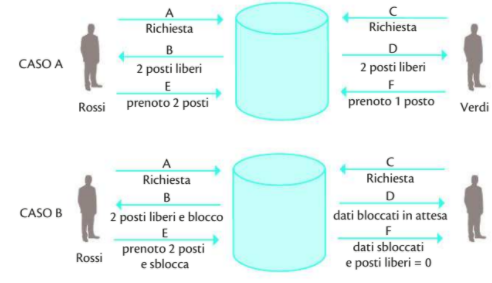
\includegraphics[scale=1.2]{acc.PNG}
    
\end{center}
\hline
\section{\underline{Progettare una base di dati}}
\subsection{La progettazione di un database}
\subsubsection{Dati e informazioni}
Per \textbf{dato} si intende un fatto raccolto tramite osservazioni e/o misurazioni.
Per \textbf{informazione} si intende l'interpretazione e il collegamento tra i Il dati.

\begin{center}
    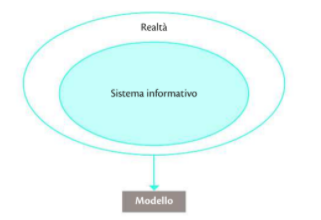
\includegraphics[scale=1.1]{mod.PNG}
\end{center}

Il modello raèèresenta una percezione di una parte della realtà,e nel processo di modellizzazione viene effettuata la selezione degli aspetti necessari per comprendere il contesto che vogliamo analizzare.

\subsubsection{Fasi della progettazione}
Il compito del DBA è quello di decidere quali parti della realtà sono inerenti per le applicazioni che utilizzeranno la base di dati.
Normalmente la progettazione è divisa in quattro fasi:

\begin{center}
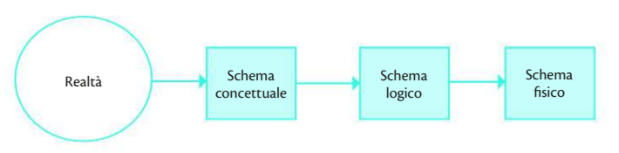
\includegraphics[scale=1.1]{fasi.PNG}
    
\end{center}


\begin{enumerate}
    \item \textbf{Raccolta e analisi dei dati}\\
    Raccolta dei requisiti del sistema informativo (dati, processi, vincoli), che vengono descritte in appositi glossari.
    \item \textbf{Progettazione concettuale}\\
    Si formalizzano le descrizioni di come gli utenti vedono i dati (viste utenti), che vengono integrate in uno schema concettuale.
    \item \textbf{Progettazione logica}\\
    Viene sviluppato uno schema logico sullo schema concettuale.
    \item \textbf{Progettazione fisica}\\
    Vengono definite le strutture di memorizzaazione e i loro parametri.
\end{enumerate}

\subsection{Il modello E/R - Entità e Attributi}

Esistono vari modi per descrivere i dati in modo indipendente dalla macchina:
\begin{itemize}
    \item \textbf{i modelli logici}
    \item \textbf{i modelli concettuali }
\end{itemize}

\subsubsection{Lo schema Entità/Relazioni}
La descrizione concettuale dei dati si basa sull'individuazione e la definizione delle entità e delle associazioni inerenti al contesto. Tramite il modello \textbf{Entità/Relazioni} che rimanendo semplice ed intuitivo può essere descritto graficamente.\\

\begin{center}
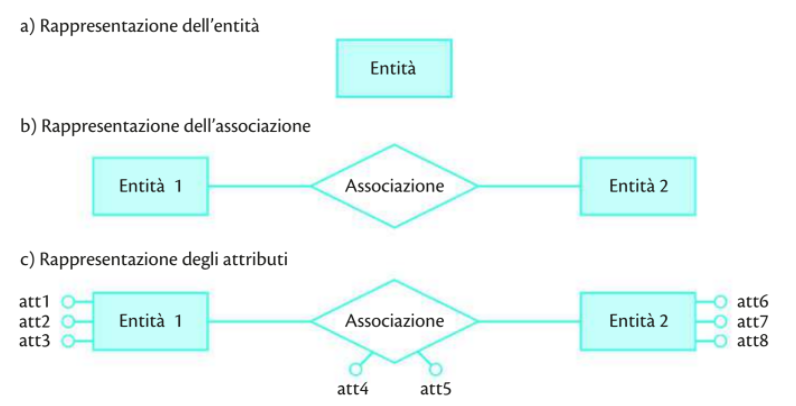
\includegraphics[scale=1.0]{er.PNG}    
\end{center}

In questo modo si può descrivere la realtà tramite delle entità e le loro associazioni.

\subsubsection{Entità}
Le entità sono elementi dotati di caratteristiche comuni, che vengono riuniti in una classe.
\\
\underline{Si chiama \textbf{istanza} dell'entità \textbf{un esemplare} della classe}.

\begin{footnotesize}
esempio:\\
\end{footnotesize}

\textbf{Studente}:\\

\begin{footnotesize}
attributi:\\
\end{footnotesize}
\textbf{ID}:4567\\
\textbf{Nome}:Mario\\
\textbf{Cognome}:Verdi\\
\textbf{Classe}:5bi\\

\subsubsection{Attributi}
\colorbox{yellow}{Gli attributi sono le proprietà che servono a descrivere le entità e le associazioni.} \\
Nello schema ER vengono rappresentati con dei punti collegati alle entità o alle associazioni. E sono identificati dal tipo, dal dominio.\\
Possono essere:
\begin{itemize}
    \item \textbf{Semplici}: che hanno un tipo semplice (es: Insegnante)
    \begin{center}
       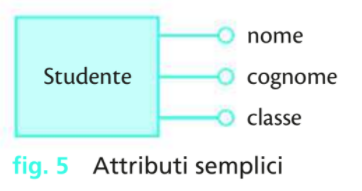
\includegraphics[h!]{att.PNG} 
    \end{center}
    
    \item \textbf{Composti}: in cui esistono sottoattributi (per esempio una data(giorno,mese,anno))

\begin{center}
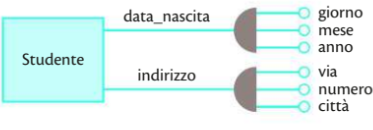
\includegraphics[h!, scale=1.2]{att-.PNG} 
\end{center}
    \item \textbf{Multipli}: esiste un numero variabile di sottoelementi dello stesso tipo (esempio:voto  scolastico).
    \begin{center}
        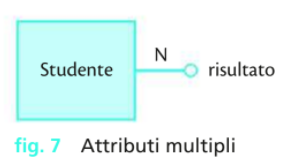
\includegraphics[]{attm.PNG}
    \end{center}
\end{itemize}

Gli attributi poi possono essere \textbf{opzionali}: se si permette che l'attributo possa non avere un valore assegnato (NOT NULL) o \textbf{obbligatori}: in cui è obbligatorio che l'attributo abbia un valore che non sia NOT NULL.
\subsection{Le chiavi}
La \textbf{chiave primaria} identifica univocamente le istanze di un entità. Nello schema ER si evidenzia dagli altri attributi perchè viene sottolineato.
\begin{center}
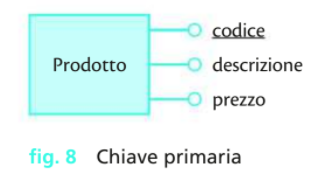
\includegraphics[]{chiave.PNG}    
\end{center}
Non possono esistere chiavi primarie con valori uguali, altrimenti non si potrebbero distinguere le istanze. In un entità ci possono essere diversi attributi \textbf{candidati}, in base al contesto viene scelta la chiave primaria più attinente.
\subsection{Le relazioni 1:1 e 1:N}
\colorbox{yellow}{Le relazioni sono i legami logici tra le entità. Si può parlare di classi di relazioni (1:1, 1:N, N:N).}\\
L'associazione viene rappresentata graficamente con un rombo che collega le entità associate.\\
\begin{center}
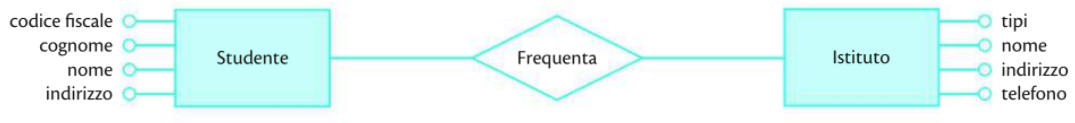
\includegraphics[scale=0.9]{ent.PNG}    
\end{center}

\subsubsection{Tipi di relazioni tra entità}

\begin{itemize}
    \item \textbf{Relazioni 1:1}:
        ad ogni elemento del primo insieme ne corrisponde uno e uno solo del secondo insieme.
    \begin{center}
    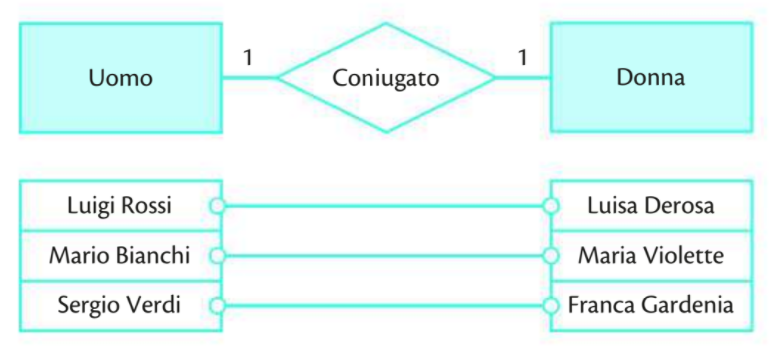
\includegraphics[scale=0.85]{11.PNG}
    \end{center}
    
    \item\textbf{Relazioni 1:N}: A un elemento del primo insieme possono corrispondere più elementi del secondo insieme, ma non viceversa.
    
    \begin{center}
        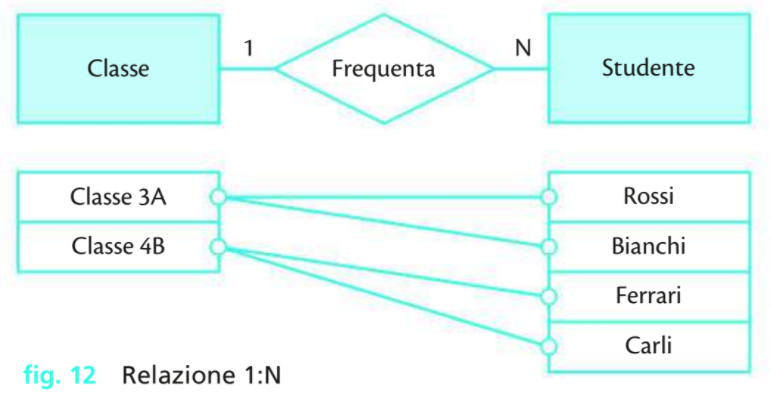
\includegraphics[scale=0.85]{1n.PNG}
    \end{center}
\end{itemize}

\subsection{Cardinalità delle associazioni}


  La cardinalità di un associazione definisce il numero di istanze con cui può partecipare un associazione. E' identificata da due numeri, che indicano la cardinalità \textbf{minima} e \textbf{massima}.\\
  \begin{center}
      
  
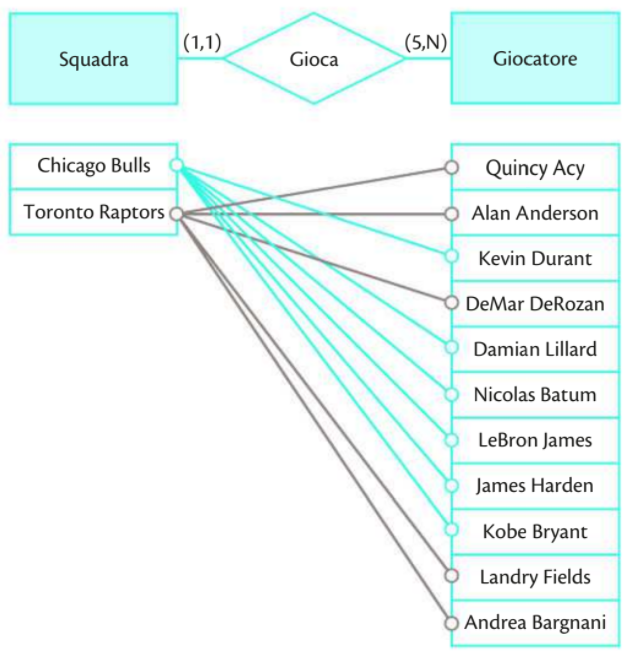
\includegraphics[scale=0.75]{ca.PNG}
\end{center}

La cardinalità minima uguale a zero indica che l'entità partecipa in \textbf{modo opzionale} all'associazione.  
\begin{center}
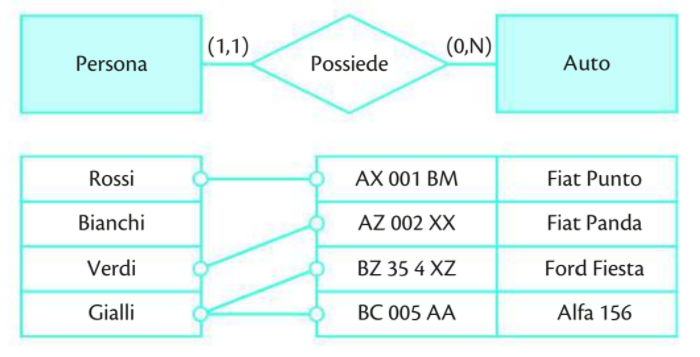
\includegraphics[]{per.PNG}    
\end{center}

\subsection{Le relazioni con N:N e le relazioni con gli attributi}
Le relazioni N:N riguardano le associazioni che coinvolgono N elementi, sia della prima che della seconda entità

\subsubsection{Associazioni com gli attributi}
\textbf{Gli attributi}, oltre a riferirsi alle entità, \textbf{possono riferirsi anche alle associazioni} se specificano una caratteristica riguardante una associazione tra due entità.\\
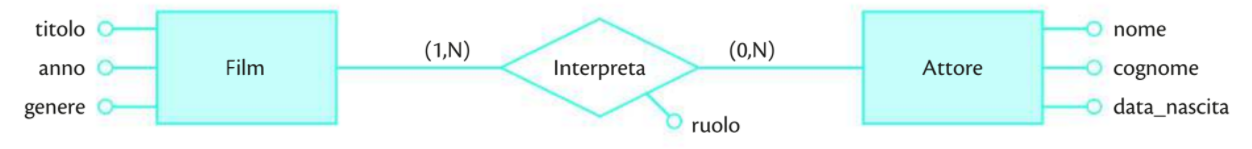
\includegraphics[scale=0.8]{as.PNG}\\
\subsection{Entità deboli con identificazione esterna. Gerarchi}

\section{\underline{Il linguaggio SQL}}
\subsection{Definire lo schema}
\textbf{SQL}(\textbf{S}tructured \textbf{Q}uery \textbf{L}anguage) è un linguaggio che ti permette di eseguire operazioni CRUD (Create, Read, Update, Delete) in basi di dati relazionali. SQL fa parte è un linguaggio \textit{\textbf{non procedurale}} in cui non devi specificare come vuoi trovare qualcosa, ma solamente cosa vuoi trovare. 

Il linguaggio SQL ha diverse categorie specializzate:
\begin{itemize}
    \item \textbf{DDL} (\textbf{D}ata \textbf{D}efinition \textbf{L}anguage): creare e modificare schemi di database 
    \item \textbf{DML} (\textbf{D}ata \textbf{M}anipulation \textbf{L}anguage): inserire, modificare e gestire dati 
    \item \textbf{DQL} (\textbf{D}ata \textbf{Q}uery \textbf{L}anguage): interrogare i dati
    \item \textbf{TCL} (\textbf{T}ransaction \textbf{C}ontrol \textbf{L}anguage): creare e gestire transazioni
    \end{itemize}
    \subsubsection{Creazione di database}
    Per creare un database si usa la seguente sintassi:\\
    CREATE DATABASE nome\_database\\
    Per eliminare un database esistente si usa il comando:\\
    DROP DATABASE nome\_database
    \subsubsection{Creazione di tabelle}
    Per creare una tabella si usa il comando CREATE TABLE:\\
    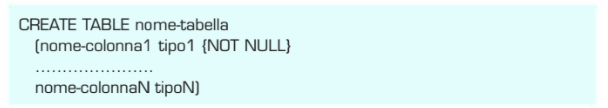
\includegraphics[]{TAB.PNG}\\
    Accanto al nome di ogni tabella deve essere specificato il tipo di dato.
    Se necessario possono essere specificate anche altre clausole:
    \begin{itemize}
        \item \textbf{NOT NULL} (il valore non può essere nullo)
        \item \textbf{PRIMARY KEY} (definisce la chiave primaria)
        \item \textbf{UNIQUE} (dice che il campo non può avere valori duplicati)
        \item \textbf{FOREIGN KEY} (definisce una chiave esterna)
    \end{itemize}
    \subsubsection{Tipi di dati}
    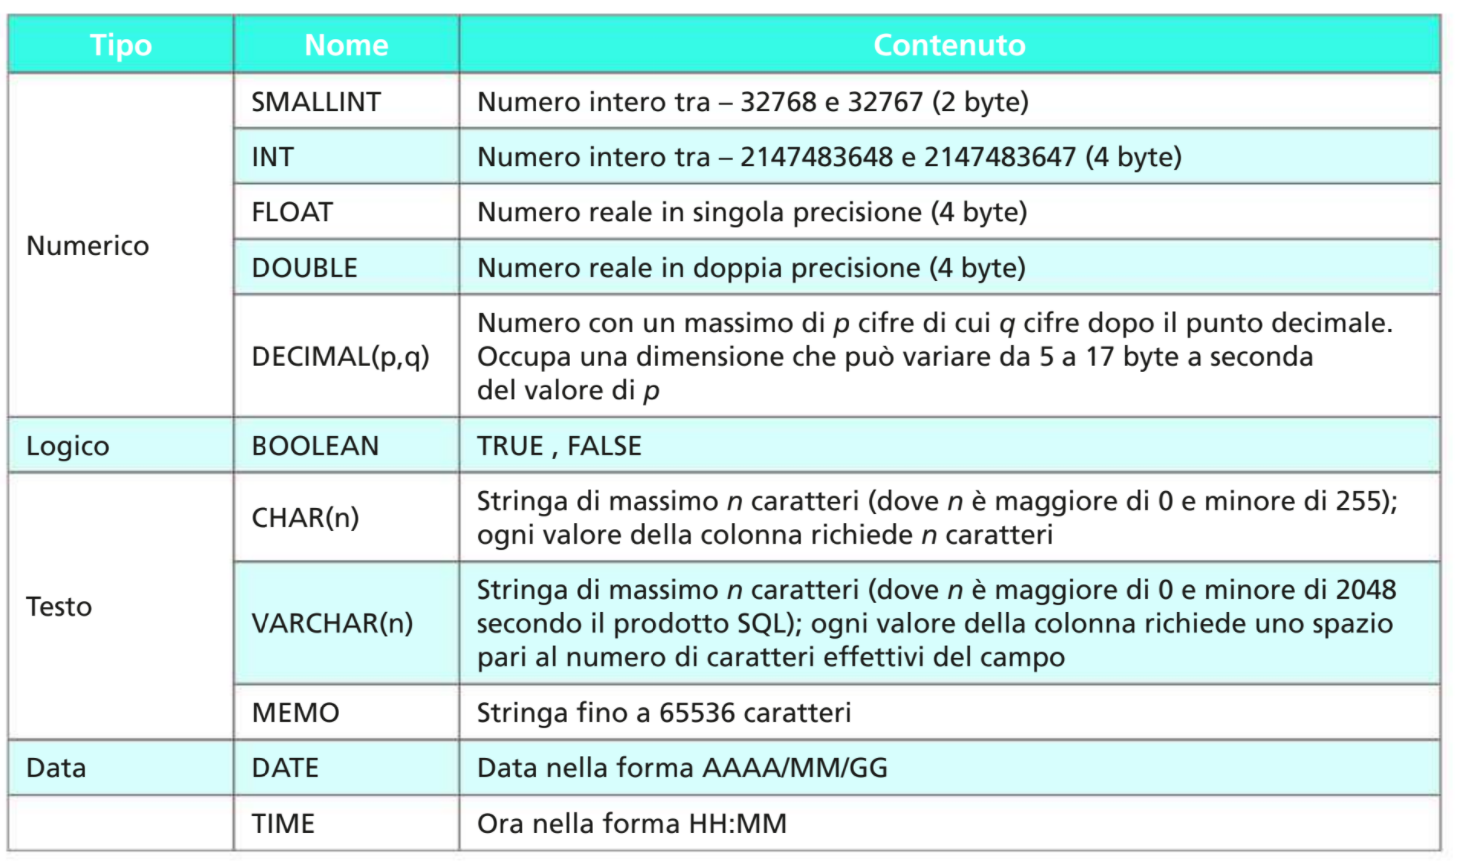
\includegraphics[scale=0.7]{dati.PNG}
    in caso espandi
    
    \subsubsection{Creare un indice}
    Per migliorare l'efficienza di ricerca delle righe nelle tabelle si definisce un indice sul campo di ricerca.
    
    Un indice su una tabella esistente si crea con l'istruzione CREATE INDEX\\
    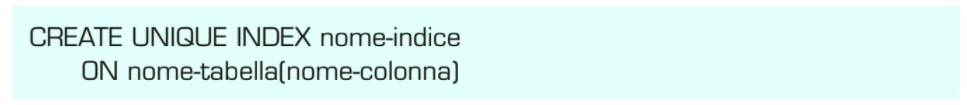
\includegraphics[scale=0.9]{index.PNG}\\
    Gli indici sono importantissimi per velocizzare le operazioni di interrogazione. Quando si aggiornano le tabelle si deve ricontrollare la validità degli indici.
    \subsection{Modificare lo schema di una base di dati}
    Lo schema dei dati può essere modificato sia eliminando tabelle o indici, sia modificando la struttura stessa della tabella.\\
    \subsubsection{ALTER TABLE}
    L'istruzione ALTER TABLE permette di modificare a struttura di una tabella. La clausola successiva indica il tipo di modifica che si vuole effettuare sulla tabella.(aggiunta, eliminazione e modifica).\\
    Per \textbf{inserire una colonna} in una tabella esistente:\\
    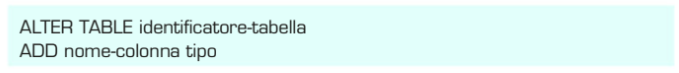
\includegraphics[scale=1.2]{at.PNG}\\
    \footnotesize{esempio:}\\
    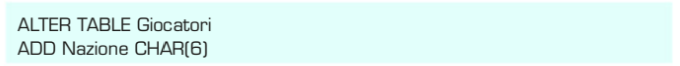
\includegraphics[scale=1.2]{esat.PNG}  \\
    Per \textbf{cancellare una colonna} da una tabella già esistente si usa:\\
    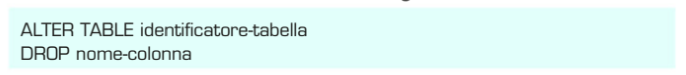
\includegraphics[scale=1.2]{atc.PNG}\\
    \footnotesize{esempio:}\\
    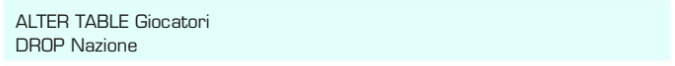
\includegraphics[scale=1.2]{esn.PNG}\\
    Per \textbf{cambiare il tipo di una colonna} si fa:\\
    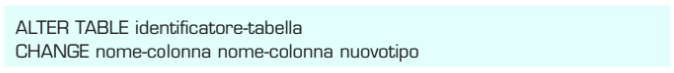
\includegraphics[scale=1.2]{modid.PNG}\\
    \footnotesize{esempio:}
    
    
    
    
    
\newpage
\section{\underline{Interrogazioni}}



\subsection{Domande professoressa}
\begin{enumerate}
    \item Informazioni all'interno aziende? 
    \item Come si arriva alla necessità delle basi di dati?
    \item Integrità e consistenza delle basi di dati?
    \item Il modello ANSI/SPARC?
    \item Quali sono le tipologie di utenti di un DBMS?
    \item Quali sono i vincoli delle basi di dati?
    \item Con che istruzione l'amministratore della base di dati assegna i permessi agli  utenti?
    \item Il modello logico relazionale per le basi di dati?
    \item Nello schema logico relazionale, da dove arrivano queste tabelle? che caratteristiche hanno i dati che ci sono dentro?
    \item Che caratteristiche che devono avere i dati nelle tabelle relazionali?
    \item Fai un esempio di una 1:N
    \item Cos'è JDBC?
    \item Cos'è il modello relazionale per le basi di dati?
    \item Cos'è SQL?
    \item Cosa sono e quali sono le cardinalità?
    \item Come si fa a togliere i permessi in un DB?
    \item Gli attributi nella progettazione ER vengono solo dalle entità? 
    \item Cosa fanno le chiavi primarie?
    \item Cosa sono le chiavi candidate?
    \item Cosa sono le chiavi surrogate?
    \item Che tipi di attributi esistono? fai degli esempi
    \item Cosa si intende per dominio?
    \item Cos'è la ristrutturazione? fai degli esempi
    \item Quali sono le fasi della progettazione concettuale? analizza ogni fase
    \item Come sono tradotte le associazioni in tabelle? Cosa differenzia la loro tradizione dalle istanze?
    \item Che vincoli devono rispettare le tabelle in un sistema relazionale?
    \item SQL- com'è strutturata la gerarchia delle Queary?
    \item Che cosa sono gli operatori aggregati? Quali sono? Dove si possono utilizzare?
    \item Qual è la differenza tra JOIN left e JOIN right?
    \item Quali sono i due conceti chiave delle Queary ( connessione e statement) 
    
\end{enumerate}

\subsection{Consigli della prof}
\begin{itemize}
    \item Parlare lentamente
    \item Non andare a infilarti in cose che non conosci
    \item Non divagare
    \item Quando parli di qualcosa fai esempi
\end{itemize}


\end{document}
